\documentclass[tikz,border=0pt]{standalone}
%\usepackage{mathptmx}
\usepackage[utf8]{inputenc}
\usetikzlibrary{patterns,decorations.pathmorphing,positioning,arrows,automata}

\begin{document}
	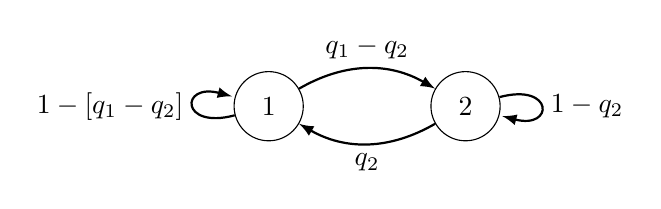
\begin{tikzpicture}[node distance=2.5cm,->,>=latex,auto,
		every edge/.append style={thick}]
		\node[state] (1) {$1$};
		\node[state] (2) [right of=1] {$2$};  
		\path (1) edge[loop left]  node{$1-[q_{1}-q_{2}]$} (1)
		edge[bend left]  node{$q_{1}-q_{2}$}   (2)
		(2) edge[loop right] node{$1-q_{2}$}  (2)
		edge[bend left] node{$q_{2}$}     (1);
	\end{tikzpicture}
\end{document}